\documentclass{beamer-control}
\usepackage{beamer-control-singlefile}
\INCLUDEONLY{Performance Specifications}
\begin{document}
\CONCEPT{Performance Specifications}

\begin{SUMMARY}
\begin{itemize}
\item Frequency domain features 
\item Response to reference signals
\item Response to disturbances and noise
\end{itemize}
\vfill References:
\begin{itemize}
\item \astrom{§12.2}
\end{itemize}
\end{SUMMARY}


\SUBCONCEPT{Frequency domain features }
\begin{frame}{Characterising performance}
	\begin{itemize}
		\item The goal of performance specificaitons are to capture the characteristic properties of a system with minimal parameters
		\item Time domain features we have seen are overshoot, rise time, and settling time
		\item In frequency domain we have peak values, peak frequnecy, gain crossover frequency, and bandwidth
		\item The maximum value of the sensitivity and complementary sensitivity functions, $M_s$ (occuring at $\omega_{ms}$) and $M_t$ (occuring at $\omega_{mt}$), are also important
		\item The sensitivity crossover frequency $\omega_{sc}$ is defined as the frequency where the magnitude of thesensitivity function is 1
	\end{itemize}
\end{frame}

\SUBCONCEPT{Response to reference signals}

\begin{frame}{Tracking specifications}
\begin{itemize}
\item The responses of the output $y$ and control signal $u$ to the reference $r$ are described by 
\[G_{yr} = \frac{PCF}{1+PC} \quad \text{and} \quad G_{ur} = \frac{CF}{1+PC}\]
\item Specifications for response to reference signals can be expressed in terms of features of $G_{yr}$ such as the peak value $M_r$, peak frequency $\omega_{mr}$, and bandwidth $\omega_b$
\end{itemize}
\begin{figure}
	\centering
	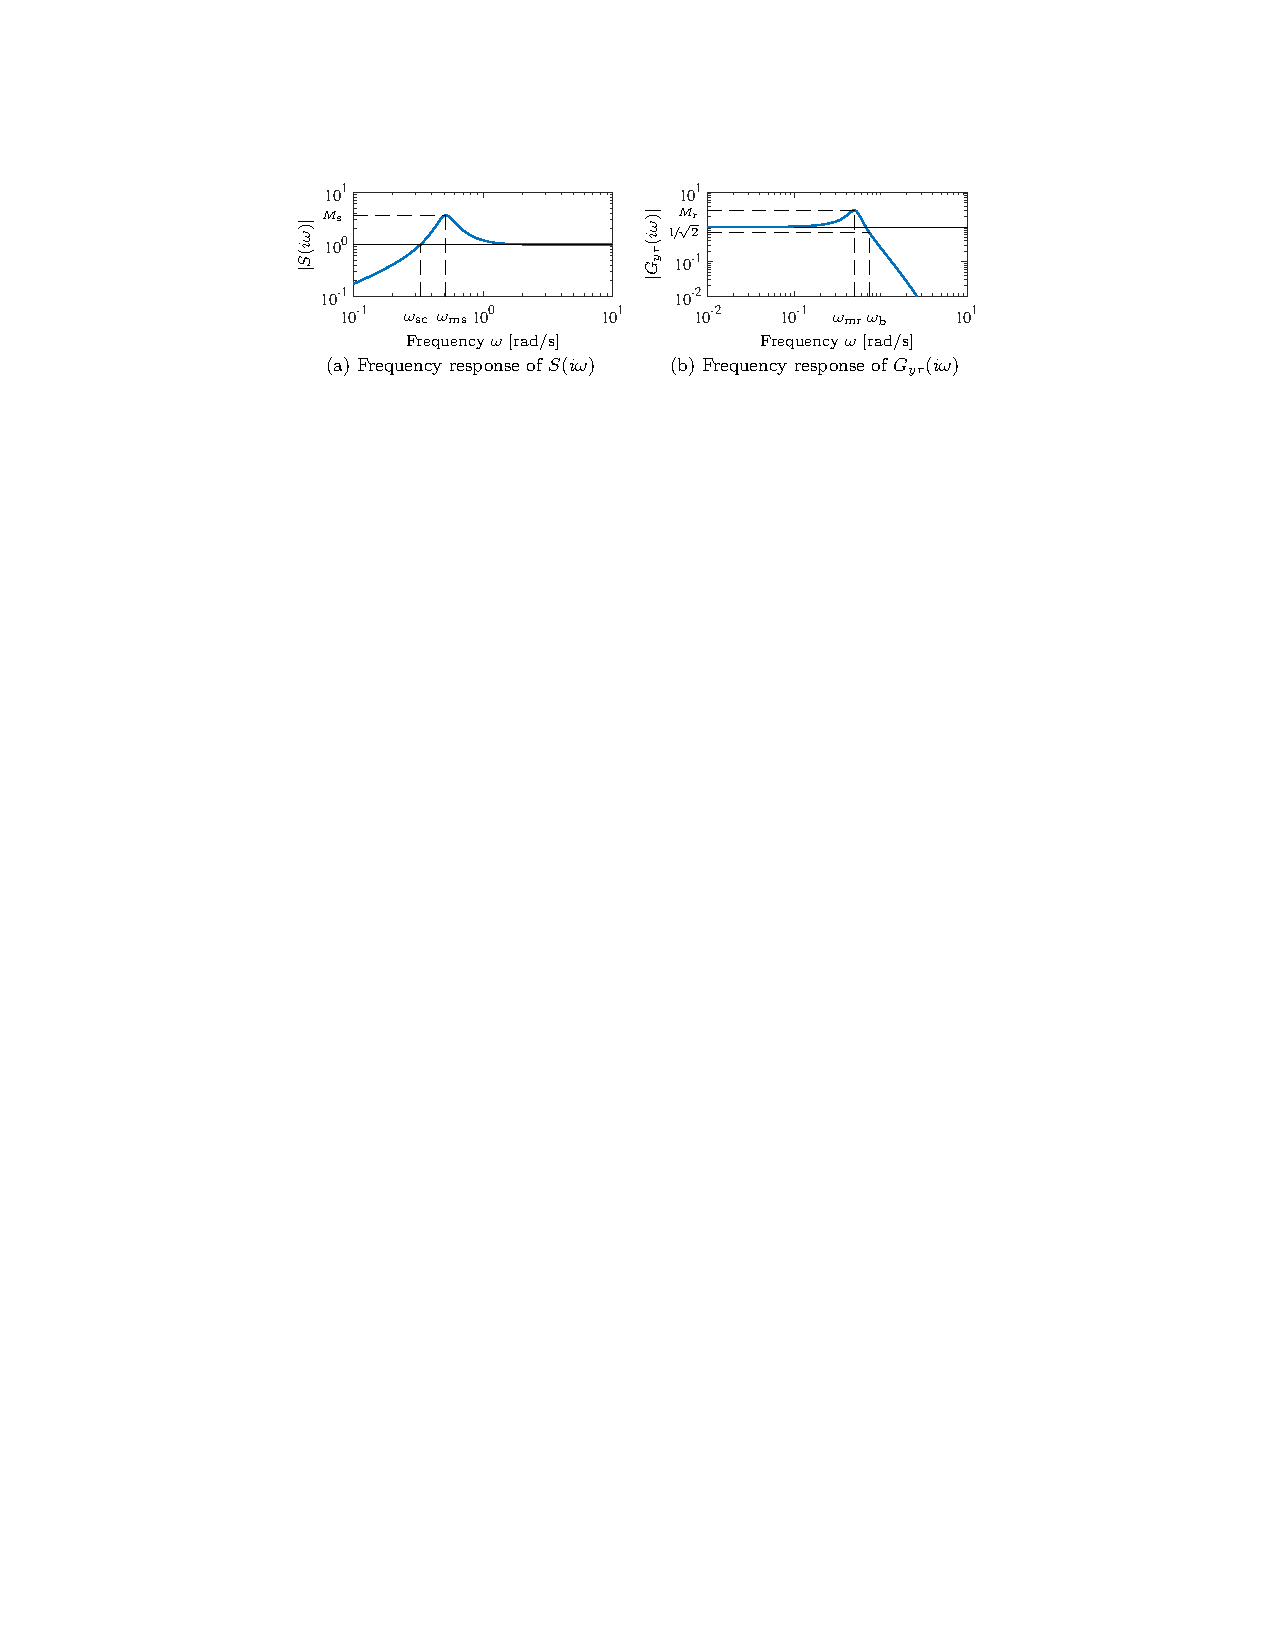
\includegraphics[width=10cm]{figure12.3}\\
	\textbf{Figure 12.3:} Illustration of specifications in frequency domain.
\end{figure}
\end{frame}


\begin{frame}{Tracking at low frequency}
	\begin{itemize}
		\item The transfer function $G_{yr}$ typically has unit zero frequency gain as we want the system to have step input with zero steady-state error
		\item The behaviour at low frequencies determines the tracking error for slow reference signals
		\item We can investigate by considering small $s$
		\[G_{er}(s)\approx e_1 s+ e_2 s^2+\cdots\]
		where $e_k$ are called error coefficients
		\item For a reference signal $r(t)$
		\[e(t)=r(t)-y(t)=G_{er} r= e_1 \frac{\mathrm{d}r}{\mathrm{d}t}+ e_2 \frac{\mathrm{d}^2r}{\mathrm{d}t^2}+ \cdots\]
		as multiplying by $s$ corresponds to differentiation in time
	\end{itemize}
\end{frame}


\begin{frame}{Low frequency $\rightarrow$ long time}
	\begin{itemize}
		\item A ramp input, $r(t)=v_0t$, therefore has a steady-state error of $v_0e_1$ and so is zero if $e_1=0$
		\item For a quadratic input, $r(t)=a_0 t^2$, a system with $e_1=0$ will have steady-state error $e(t)=2ae_2$
		\item The behaviour at low frequencies (small $s$) corresponds to behaviour at large times (steady-state performance)
	\end{itemize}
\end{frame}




\begin{frame}{Example}
\begin{itemize}
	\item Consider a process with transfer function $P(s)=\frac{1}{(s+1)^3}$
	and a PI controller with error feedback having gains $k_p=0.6$ and $k_i=0.5$
	\item We compare the performance of a controller with only error feedback, and  with feedforward control implemented
\end{itemize}
\begin{figure}
	\centering
	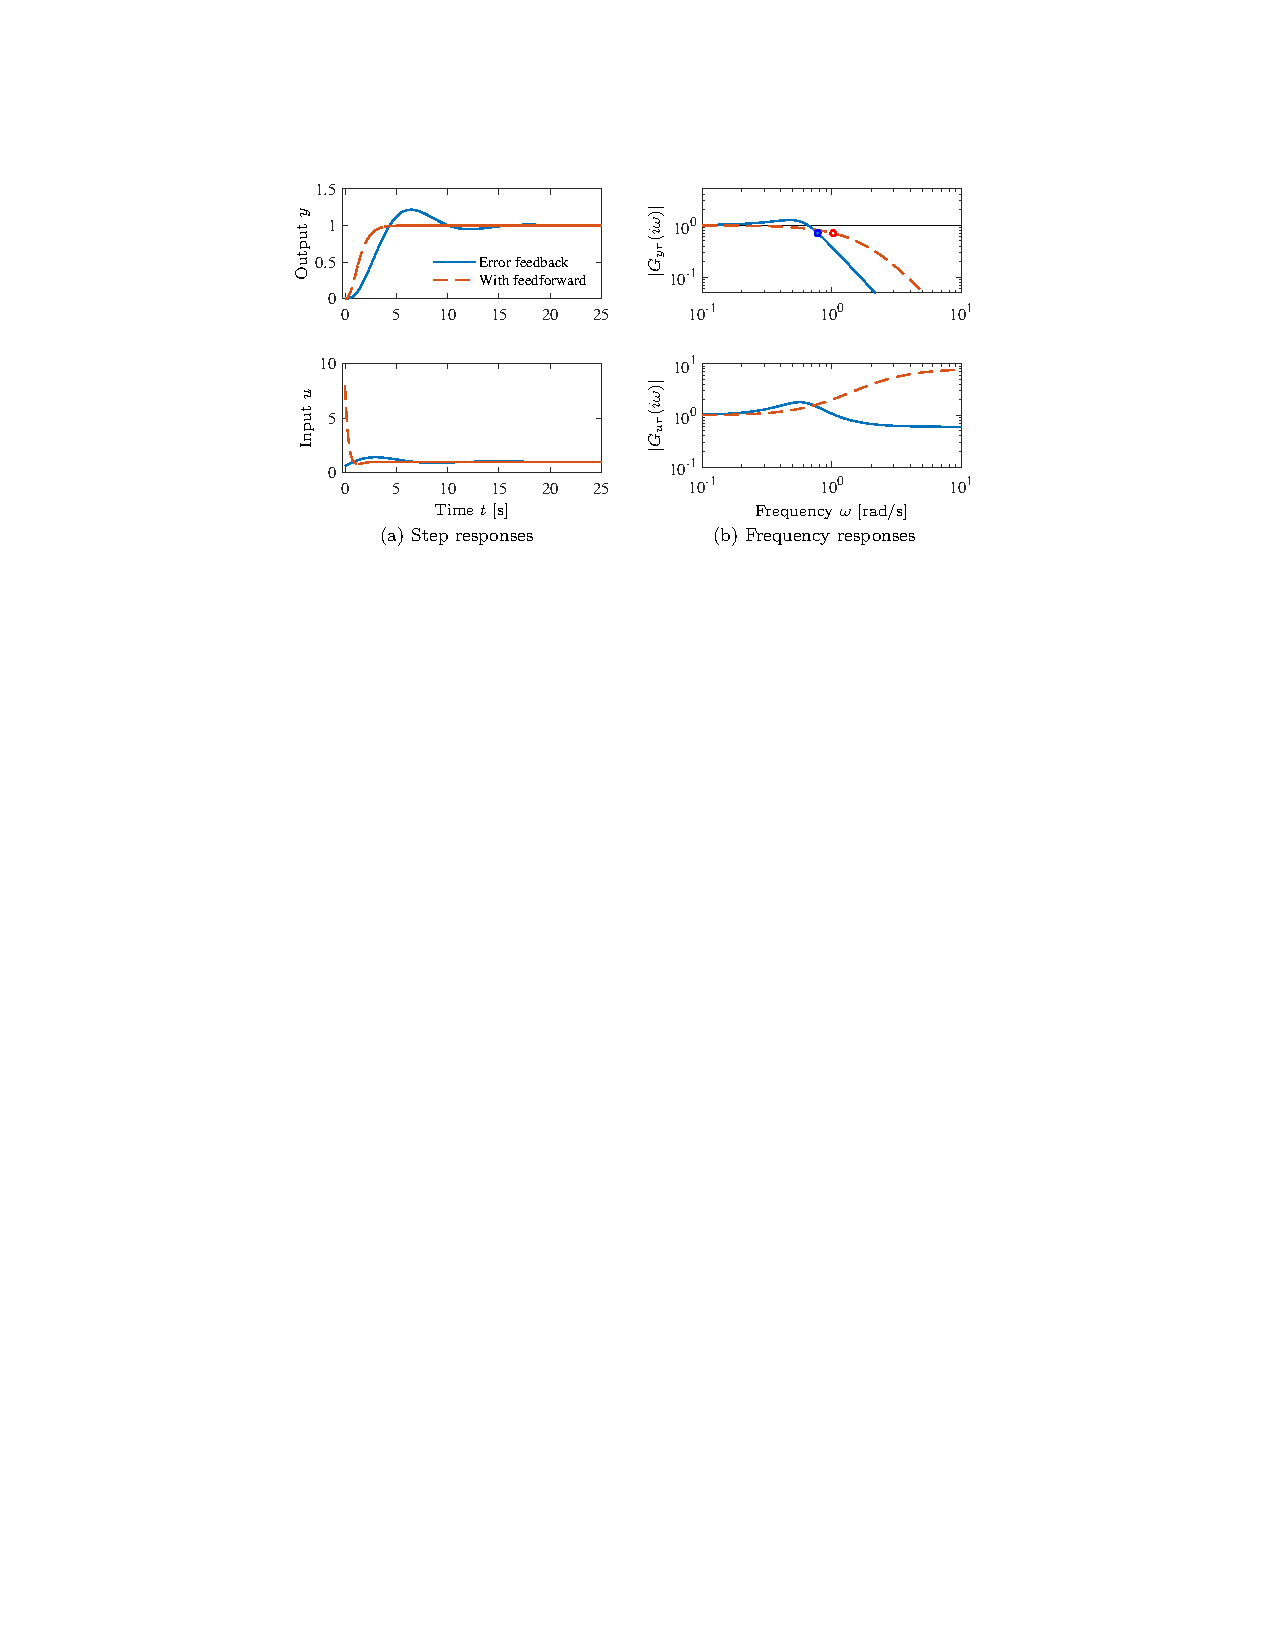
\includegraphics[width=8cm]{figure12.4}\\
	\vspace{-0.2cm}
	\textbf{Figure 12.4:} Responses to unit step.
\end{figure}
\end{frame}


\begin{frame}{Example continued}
\begin{itemize}
	\item The feedforward controller has a faster response with no overshoot but requires larger control signals
	\item The feedforward controller has larger bandwidth indicated by the circles in Figure 12.4(b) and no resonant peak
	\item We can glean some insight here...
	\item Large overshoots in time responses correspond to large resonant peaks in the frequency response
	\item The product of the rise time of the unit step response and the bandwidth of a transfer function (the rise time-bandwidth product) is a useful characteristic 
	\item It is often approximately constant ($T_r\omega_b\approx 3$) and hence rise time may be inferred from bandwidth
\end{itemize}
\end{frame}

\SUBCONCEPT{Response to disturbances and noise}

\begin{frame}{The sensitivity function}
\begin{itemize}
\item The sensitivity function $S$ shows how feedback influences the reponse of the output to both load disturbances and measurement noise
\item Disturbances with frequencies such that $|S(i\omega)|<1$ are attenuated and disturbances with frequencies with $|S(i\omega)|>1$ are amplified by feedback
\item The sensitivity crossover frequency $\omega_{sc}$ is the lowest frequency where $|S(i\omega)=1$
\end{itemize}
\end{frame}

\begin{frame}{Relation to Nyquist}
\begin{itemize}
	\item As we have $S=\tfrac{1}{1+L}$, disturbance rejection can be visualised on a Nyquist plot of the loop transfer function
	\item The complex number $1+L(i\omega)$ is the inverse of $S(i\omega)$ and can be viewed as the vector from $-1$ to the point $L(i\omega)$ on the Nyquist curve
	\item The sensitivity is less than 1 for points outside a circle with radius 1 centred at -1 (attenuation of disturbances)
\end{itemize}
\begin{figure}
	\centering
	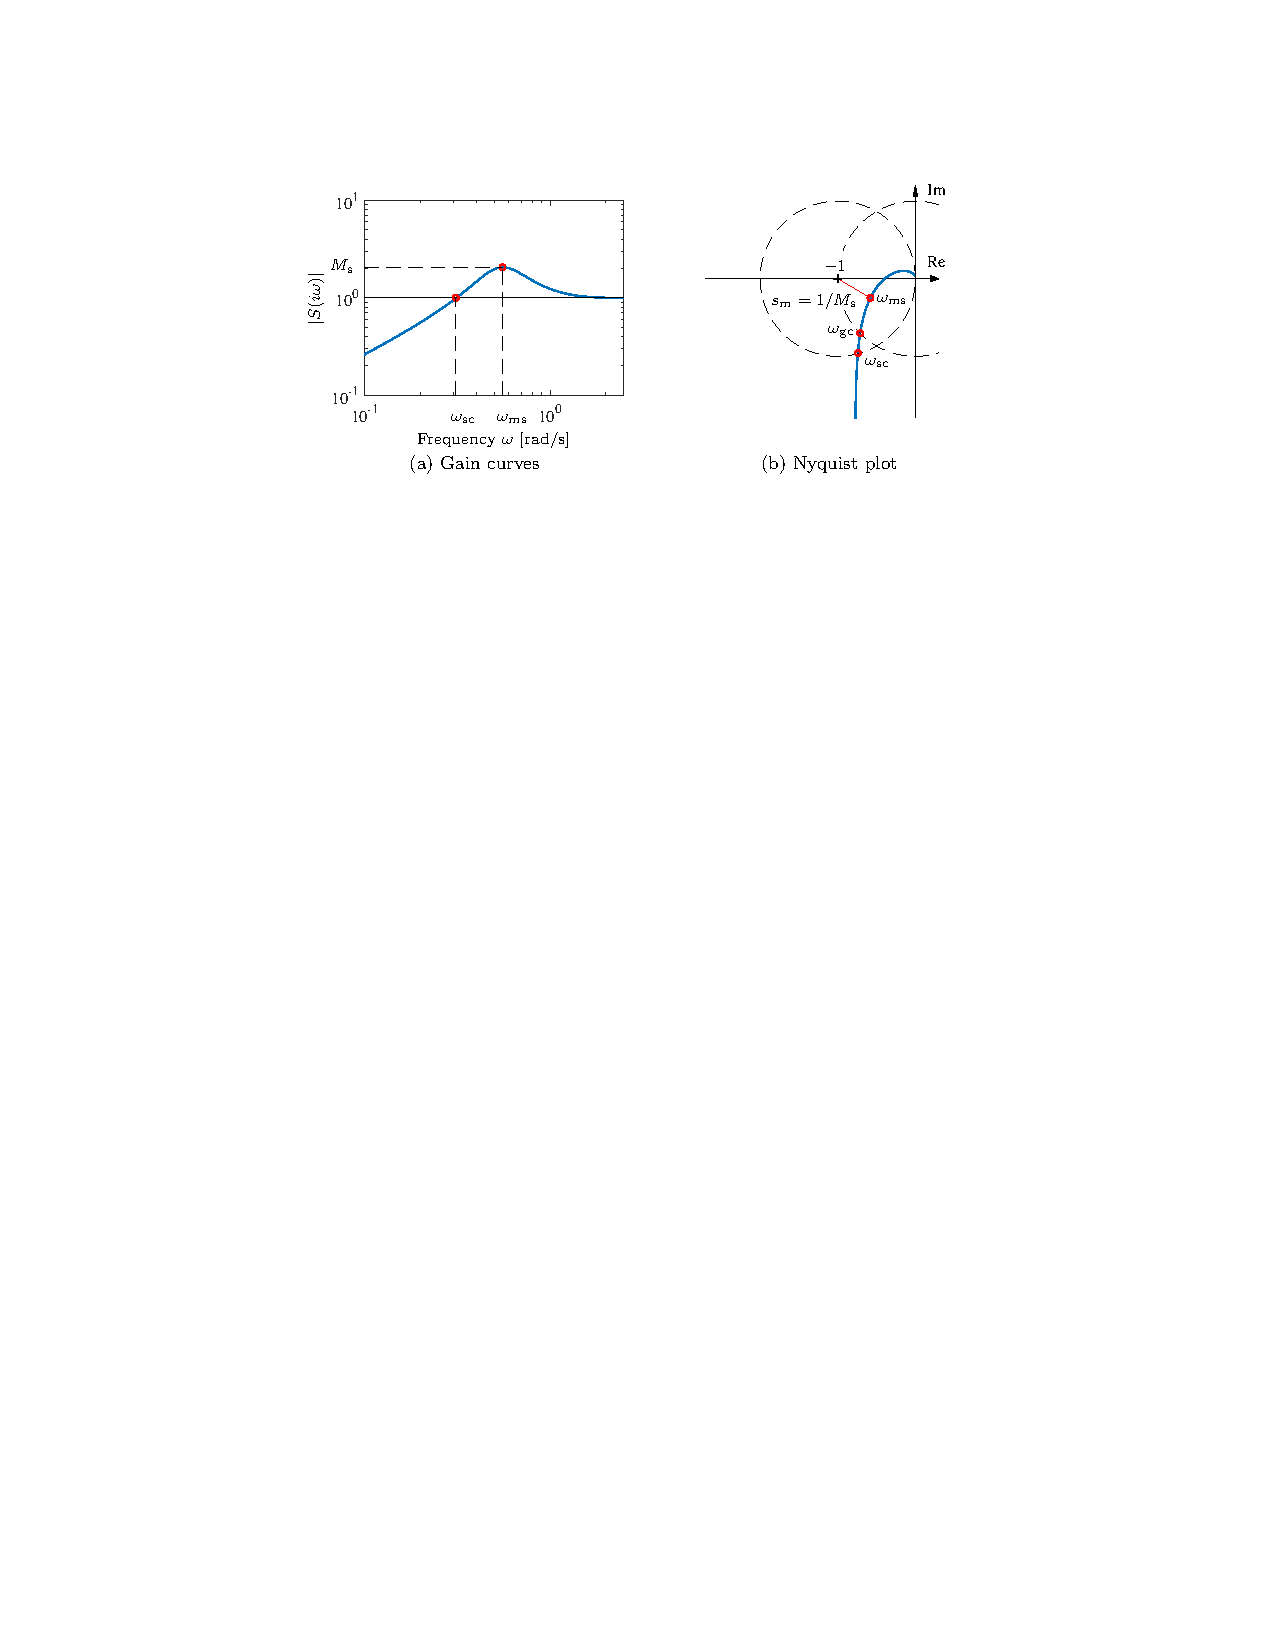
\includegraphics[width=8cm]{figure12.5}\\
	\vspace{-0.2cm}
	\textbf{Figure 12.5:} Illustration of sensitivity to disturbances.
\end{figure}
\end{frame}


\begin{frame}{Maximum sensitivity}
\begin{itemize}
	\item The maximum sensitivity $M_s$ (which occurs at $\omega_{ms}$ is a measure of the largest amplification of disturbances
	\item It is equal to the inverse of the stability margin
	\[M_s=\frac{1}{s_m}\]
	\item The sensitivity crossover frequency $\omega_{sc}$ and the maximum sensitivity $M_s$ give a characterisation of load disturbance attenuation
\end{itemize}
\end{frame}

\begin{frame}{Load disturbance transfer function}
	\begin{itemize}
		\item The transfer function from load disturbance $v$ to process output $y$ is 
		\[G_{yv} = \frac{P}{1+PC}=PS=\frac{T}{C}\]
		\item As load disturbances typically have low frequencies, small $s$ results in $T\approx1$ and so $G_{yv}\approx \frac{1}{C}$
		\item Therefore, for a controller with integral action at small $s$, $G_{yv}\approx \frac{s}{k_i}$ and so disturbances are attenuated effectively
		
	\end{itemize}
\end{frame}

\begin{frame}{Measurement noise transfer function}
	\begin{itemize}
		\item Measurement noise is typically high frequency and therefore introduces rapid variation in the control signal
		\item The transfer function from measurement noise $w$ to control signal $u$ is 
		\[-G_{uw} = \frac{C}{1+PC}=CS=\frac{T}{P}\]
		\item Assuming that $S\approx 1$ for large $s$ (high frequencies), $-G_{uw}\approx C$
		\item Therefore, filtering the derivative so that the controller transfer function goes to zero for large $s$ is useful to keep variations in control signal reasonable
		
	\end{itemize}
\end{frame}


\SUMMARYFRAME
\FINALE

\end{document}
